\section{Practicals}
Gathering some interesting/important questions from the practicals and old exams.
\subsection{Color spaces}
\subsubsection{General parameters in color spaces}
\begin{itemize}
	\item \textbf{Chromaticity}: the color component regardless of its luminance/intensity. For example, the $xy$-diagram in Figure~\ref{fig:rgb_color_wavelength_distribution_XYZ_diagram} visualizes the chromaticity (includes saturation and hue)
	\item \textbf{Saturation}: defined as ``colorfulness of a stimulus relative to its own brightness''. In the normalized $rgb$ space, it is the distance to the point $(1/3,1/3,1/3)$ (ratio to the maximum distance). In case of the wavelength distribution, a color is saturated if it is very peaked.
	\item \textbf{Intensity}: the energy of the light. It is the integral of the wavelength distribution.
	\begin{figure}[ht!]
		\centering
		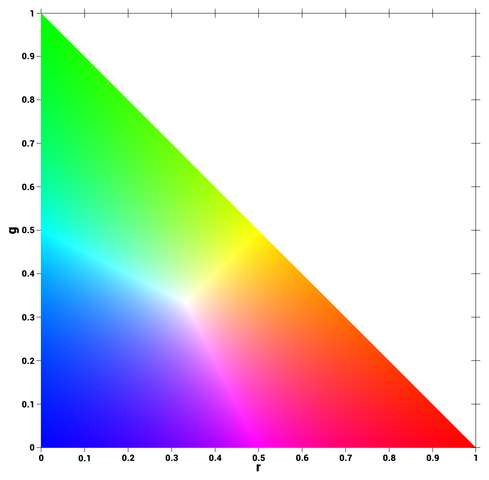
\includegraphics[width=0.25\textwidth]{figures/cv_image_formation_rg_chromaticity.png}
		\caption{\textit{rg}-chromaticity diagram. A point in this space symbolizes the chromaticity (color without intensity), and the distance to the point $(1/3,1/3)$ (if considered white light source as reference) with ratio to distance to border the saturation.}
	\end{figure}
\end{itemize}
\subsubsection{XYZ color space}
Calculate saturation, hue, intensity, plotting in the diagram, using reference lights, etc.

Interpolate between colors. We can perceive color (e.g. white) although it is not as we would define 
\subsubsection{Color invariance}
How to determine whether formula is color invariant or not. 
\begin{itemize}
	\item Color invariance is trying to remove transformations that do not directly affect the color, but let the sensor perceive it differently. 
	\item Hence, color invariant models are more or less insensitive to varying imaging conditions such as variations in illumination (light source) and object pose (shading, highlighting cues)
	\item For example, if we assume a Lambertian world where we only have body reflection and a white light source (equal for all wavelengths), we get for the $rgb$ space (note that $R=cos\theta \cdot e\cdot \int_{\lambda} p(\lambda) f_R(\lambda)d\lambda$):
	\begin{equation*}
		\begin{split}
			r & = \frac{R}{R + G + B} = \frac{\cancel{cos\theta} \cdot \cancel{e}\cdot \int_{\lambda} p(\lambda) f_R(\lambda)d\lambda}{\cancel{cos\theta} \cdot \cancel{e}\cdot \int_{\lambda} p(\lambda) \left(f_R(\lambda) + f_G(\lambda) + f_B(\lambda)\right)d\lambda}
		\end{split}
	\end{equation*}
	Thus, the \textit{rgb} color space is color invariant when assuming a Lambertian reflection model.
\end{itemize}
\subsection{Convolution operator}
\subsubsection{Difference between convolution and correlation}
Formally, correlation is a measurement of similarity between two signals whilst convolution is a measures the effect of one signal on the other. In practice however, correlation simply moves the filter over the image and computes the sum of the box at each pixel. Convolution is practically the same however before moving over the image, the filter is rotated 180 degrees. The formulas are:
\begin{equation*}
	\begin{split}
		\text{Correlation:} & I_{out} = I \otimes h,\hspace{1mm} I_{out}(i,j) = \sum\limits_{k,l} I(i+k, j+l) \cdot h(k,l)\\
		\text{Convolution:} &  I_{out} = I \ast h,\hspace{1mm} I_{out}(i,j) = \sum\limits_{k,l} I(i-k, j-l) \cdot h(k,l)
	\end{split}
\end{equation*}
Note that for both methods there is no difference in the result if we take the center pixel or a corner pixel as the start point for a filter. 
\subsubsection{Convolving two filters}
Two consecutive filters applied to an image can be summarized into one by convolving two filters. There are two ways to calculate the convolution of two filters. The more intuitive way to calculate the effect of every element of the second filter based on the first one.
Example:
\begin{equation*}
	\begin{split}
		f &=\left[\begin{array}{ccc}3 & 7 & 6\end{array}\right], \hspace{2mm}g=\left[\begin{array}{ccc}-1 & 5 & 8\end{array}\right] \Rightarrow f\ast g \\[5pt]
		& \implies \begin{array}{cccccc}
			& [-1\cdot 3 & 5\cdot 3 & 8\cdot 3] & & \\
		 +	& & [-1\cdot 7 & 5\cdot 7 & 8\cdot 7] & \\
		 +	& & & [-1\cdot 6 & 5\cdot 6 & 8\cdot 6] \\[5pt]
		 \hline
		 & [ -3 & 8 & 53 & 86 & 48 ]
		\end{array}
	\end{split}
\end{equation*}
The second option is to apply convolution right away with extended zero padding. We can imagine to use infinite zero padding but remove the zero elements in the convolved filter again. Note that we perform convolution, and therefore have to flip the second filter.
\begin{equation*}
	\begin{split}
		f\ast g & = \left[\begin{array}{ccccccc}0 & 0 & 3 & 7 & 6 & 0 & 0\end{array}\right] \otimes \left[\begin{array}{ccc}8 & 5 & -1\end{array}\right]\\
		& = \left[\begin{array}{ccccccc}-1\cdot 3 & (5\cdot 3 - 1\cdot 7) & (8\cdot 3 + 5\cdot 7 - 1\cdot 6) & (8\cdot 7 + 5\cdot 6) & 8\cdot 6\end{array}\right]\\
		& = \left[\begin{array}{ccccc}-3 & 8 & 53 & 86 & 48\end{array}\right]
	\end{split}
\end{equation*}
\subsubsection{Linearly Separable Filters}
Some 2D filters are separable in their $x$ and $y$ dimension. We can test it by comparing the convolution of separated $x$ and $y$ filters with the 2D version.
\begin{itemize}
	\item \textit{What is the benefit of separable filters?}
	
	\underline{Answer}: The computational cost is reduced form $k^2$ to $2\cdot k$.
	
	\item \textit{Prove that a 2D Gaussian filter is linearly separable.}
	
	\underline{Answer}: We can show this holds for the continuous case, and thus also for the discrete. Note that we can neglect a constant factor $c$ for normalization as this does not introduce any significant computational effort.
	\begin{equation*}
		\begin{split}
			G_x * G_y  & = \frac{1}{\sqrt{2\pi}\sigma} e^{-\frac{x^2}{2\sigma^2}} * \frac{1}{\sqrt{2\pi}\sigma} e^{-\frac{y^2}{2\sigma^2}}\\
			& = \frac{1}{2\pi\sigma^2} e^{-\frac{x^2 + y^2}{2\sigma^2}}\\
			& = G_{xy}
		\end{split}
	\end{equation*}
	\item \textit{Prove that a 2D box filter (size $3\times 3$) is linearly separable.}
	
	\underline{Answer}: We can show this by simply computing the convolution.
	\begin{equation*}
	\begin{split}
		\left[\begin{array}{ccc}1 & 1 & 1\end{array}\right] *  
		\left[\begin{array}{c}1 \\ 1 \\ 1\end{array}\right] & = \left[\begin{array}{ccc}
		1 & 1 & 1\\ 1 & 1 & 1\\ 1 & 1 & 1
		\end{array}\right]\\
	\end{split}
	\end{equation*}
	\item \textit{Check whether the following 2D filter is linearly separable:}
	$$h = \left[\begin{array}{ccc}
	1 & -2 & 1\\ -2 & 4 & -2\\ 1 & -2 & 1
	\end{array}\right]$$
	
	\underline{Answer}: The way to check that is looking for symmetric patterns in $x$ and $y$ direction which are independent of the other dimension. In this case, we can easily spot the pattern:
	\begin{equation*}
	\begin{split}
	\left[\begin{array}{ccc}1 & -2 & 1\end{array}\right] *  
	\left[\begin{array}{c}1 \\ -2 \\ 1\end{array}\right] & = \left[\begin{array}{ccc}
	1 & -2 & 1\\ -2 & 4 & -2\\ 1 & -2 & 1
	\end{array}\right]\\
	\end{split}
	\end{equation*}
	\item \textit{Check whether the following 2D filter is linearly separable:}
	$$h = \left[\begin{array}{ccc}
	1 & 8 & 3\\ 7 & 6 & 2\\ 4 & 9 & 5
	\end{array}\right]$$
	
	\underline{Answer}:  No, this kernel is not linearly separable.
\end{itemize}
\subsection{Object detection}

\subsection{Convolutional Neural Networks}
\subsubsection{Amount of parameters, output size and computational cost}
\begin{itemize}
	\item \textbf{Output size}: the spatial output size of a convolutional layer depends on the kernel size $k$, the padding $p$ (per side), the stride $s$ and the input size $w_i$. The output size is then calculated by $w_o = (w_i + 2\cdot p - k)/s + 1$
	\begin{itemize}
		\item \textit{What is the size of the output volume with stride $3$, kernel $5\times 5$, number of neurons $5$ and input size $32\times 32\times 3$ (no padding)?}
		
		\underline{Answer}: The output size is $w_0 = (32 + 2\cdot 0 - 5)/3 + 1 = 10$.
		
		\item \textit{What padding size is required to keep the output size equals to the input size for a kernel $k$ and stride $s$?}
		
		\underline{Answer}: we have to reverse the equation above to:
		\begin{equation*}
			\begin{split}
				w_o = w_i & = (w_i + 2\cdot p - k)/s + 1\\
				\Leftrightarrow (w_i - 1) \cdot s & = w_i + 2\cdot p - k\\
				\Leftrightarrow p & = \frac{1}{2}\left(w_i \cdot \left(s-1\right) - s + k\right)
			\end{split}
		\end{equation*}
		Hence, if stride is $s=1$, the necessary padding is $p=\frac{k-1}{2}$.
		
		\item \textit{How many output frames do we get for a 3D convolution of $3\times 3\times 3$ (stride $s=3$ and padding $p=1$ in temporal dimension) on a input video size of $16\times 256\times 256\times 3$?}
		
		\underline{Answer}: We can apply the same formula as before: $l_o = (16 + 2\cdot 1 - 3)/3 + 1 = 6$ output frames.
	\end{itemize}
	\item \textbf{Number of parameters}: a 2D convolution contains $k\times k\times c_F \times c_G$ parameters where $k$ is the kernel size, and $c_F$ and $c_G$ the number of input and output channels. For a 3D convolution, we multiply it by another $k$. Note that all these three $k$'s can be different (e.g. $3\times 3\times 1$, $5\times 1 \times 1$, ...)
	\begin{itemize}
		\item \textit{How many parameters are learned in a convolutional layer with an RGB input image, $5\times 5$ kernel size and $100$ different filters?}
		
		\underline{Answer}: We learn $5\times 5\times 3\times 100 = 7,500$ parameters for the filters, and $100$ biases. Thus, we have overall $7,600$ parameters.
		
		\item \textit{How many parameters are learned if we set the padding to $p=2$ and stride $s=2$?}

		\underline{Answer}: The number of parameters is independent of the stride and the padding.
	\end{itemize}
	\item \textbf{Computational cost}: The computational cost of a layer is the cost of a single filter application (the filter size) times the number of output neurons.
	\begin{itemize}
		\item \textit{Given the input $w_F \times h_F \times c_F$ and output $w_G \times h_G \times c_G$, what is the computational cost of a 2D convolution with kernel size $k\times k$ between these two layers?}
		
		\underline{Answer}: The cost of applying a single filter once is $k\times k\times c_F$. We then have to move the filter over $x$ and $y$ dimension, and repeat it for $c_G$ filters. Thus, the overall cost is determined by:
		$$k\times k\times c_F\times c_G\times w_G\times h_G$$
		
		\item \textit{Given the input $256 \times 256 \times 3$, what is the computational cost of a 2D convolution with kernel size $7\times 7$, $32$ output channels, stride $s=3$ and padding $p=0$?}
		
		\underline{Answer}: We first have to calculate the output size $w_G = (w_F + 2\cdot p - k)/s + 1 = (256 + 0 - 7)/3 = 83$ and $h_G = 83$. Next, we can apply our previous formula:
		$7\times 7\times 3\times 32\times 83\times 83$
		
		\item \textit{What are two ways to reduce the number of computations for 2D convolutions?}
		
		\underline{Answer}: Same as in case of 3D convolutions. We can either do depth-wise convolutions (\textit{MobileNet}), or do pseudo 2D convolutions by separating the filter $k\times k$ to a $1\times k$ and $k\times 1$ convolution (\textit{InceptionV2}).
	\end{itemize}
\end{itemize}
\subsubsection{Other general questions}
\begin{itemize}
	\item \textbf{Locally constrained layer}: A convolutional layer where we don't share weights over spatial dimensions.
	\begin{itemize}
		\item \textit{How many parameters are needed for a locally constrained layer, where each neuron looks at a $10\times10$ window, when using $W=H=100$, and stride of $5$?}
		
		\underline{Answer}: The spatial output size is $(100 - 10) / 5 + 1 = 19$ so that we have $19\times 19=361$ different kernels. Combined with the kernel/window size, we get overall $10\times 10\times 361=36,100$ parameters.
		\item \textit{Describe a scenario where weight sharing as done in plain convolutional layers is not beneficial for recognition}
		
		\underline{Answer}: Weight sharing works most effectively, if the input is transitional invariant. However, if this is not the case and we have stationary data, we should for example use locally constrained layers where the weights are not shared. This may lead to more parameters but reduces the required amount of channels (restricted number of possible objects per position). Example: face recognition with standardized position (eyes and mouth filters at different parts of the image). 
	\end{itemize}
\end{itemize}
